
\chapter{Introduction} 
\thispagestyle{myheadings} 
In this chapter, we first discuss some regular types of sensing systems 
used for guarding, tracking or surveilence, 
with a focus on the line-based and range-based sensors. 
These will serve as the motivation of this dissertation study
% and we then introduce the two types of simplified sensing model studied in this thesis, 
Then, we conduct a literature study of the related work on sensor placement and 
coverage related problems. 
Lastly, some background knowledge of the theories and tools used in this paper will be given. 

\section{Motivations} 
Sensor systems are ubiquitous in the modern world. 
To list a few, systems of radar antennas 
or other sensor sources are frequently used as base stations for signal transmission, 
or intruder detection system (IDS) for monitoring hazards. 
Early intruder defense system can date back to ancient times, where 
watchtowers of the Great Wall of China are used as signal points. 
It can be seen as sensors from the broad sense 
since ancient soldiers lit woods to create smoke and inform others when invaders appear. 
% Surveilence or tracking cameras surveillance and tracking system, 
\begin{figure}[ht]
    \centering 
    \begin{subfigure}[b]{0.281\textwidth} 
        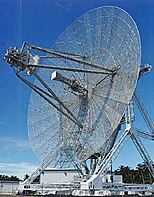
\includegraphics[width=\textwidth]{figures/Radar_antenna.jpg} 
        \caption{Radar antenna} 
        \label{fig:intro-radar} 
    \end{subfigure} 
    \begin{subfigure}[b]{0.48\textwidth} 
        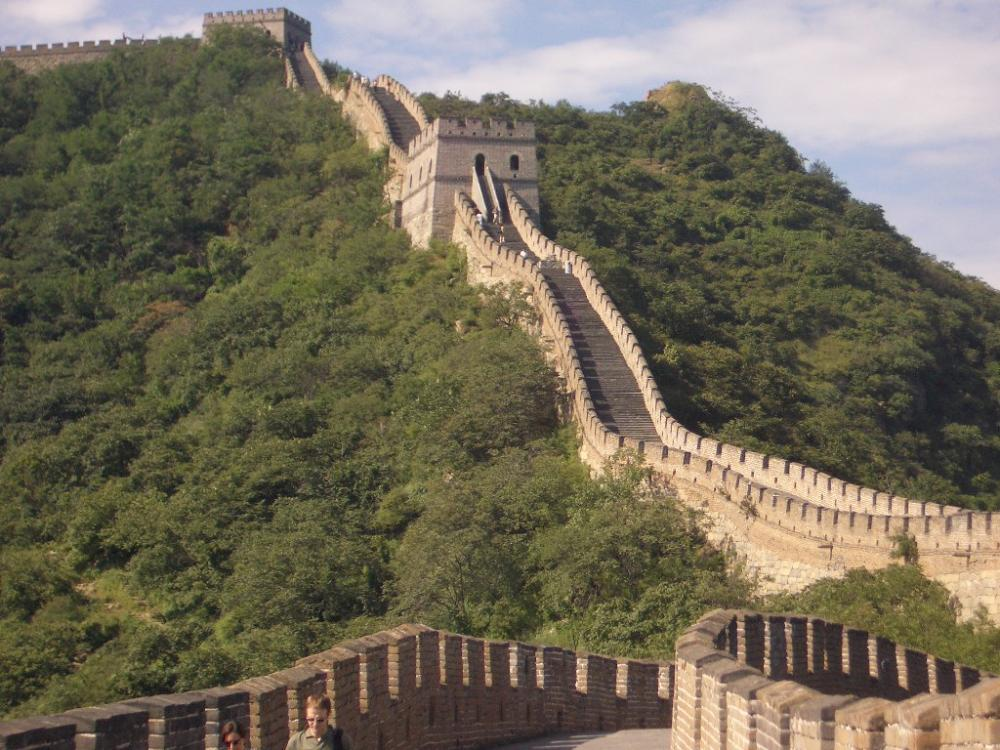
\includegraphics[width=\textwidth]{figures/great_wall.jpg} 
        \caption{Watch towers on the great wall} 
        \label{fig:intro-great_wall} 
    \end{subfigure}
    \caption{Two examples of intrusion detection system}
    \label{fig:intro-IDS}
\end{figure} 

In surveilence or tracking systems (\ref{fig:intro-laser}), 
sensors like laser beams or cameras are deployed for purposes like thief detection, 
motion capture, pose tracking and so on. 
\begin{figure}[ht] 
    \centering 
    
    % \begin{subfigure}[b]{0.55\textwidth} 
    %     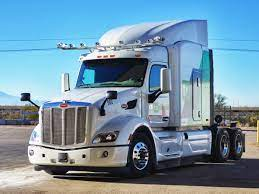
\includegraphics[width=\textwidth]{figures/truck_cam.jpeg} 
    %     \caption{Autonomous truck camera system} 
    %     \label{fig:intro_truckcam} 
    % \end{subfigure} 
    \begin{subfigure}[b]{0.41\textwidth} 
        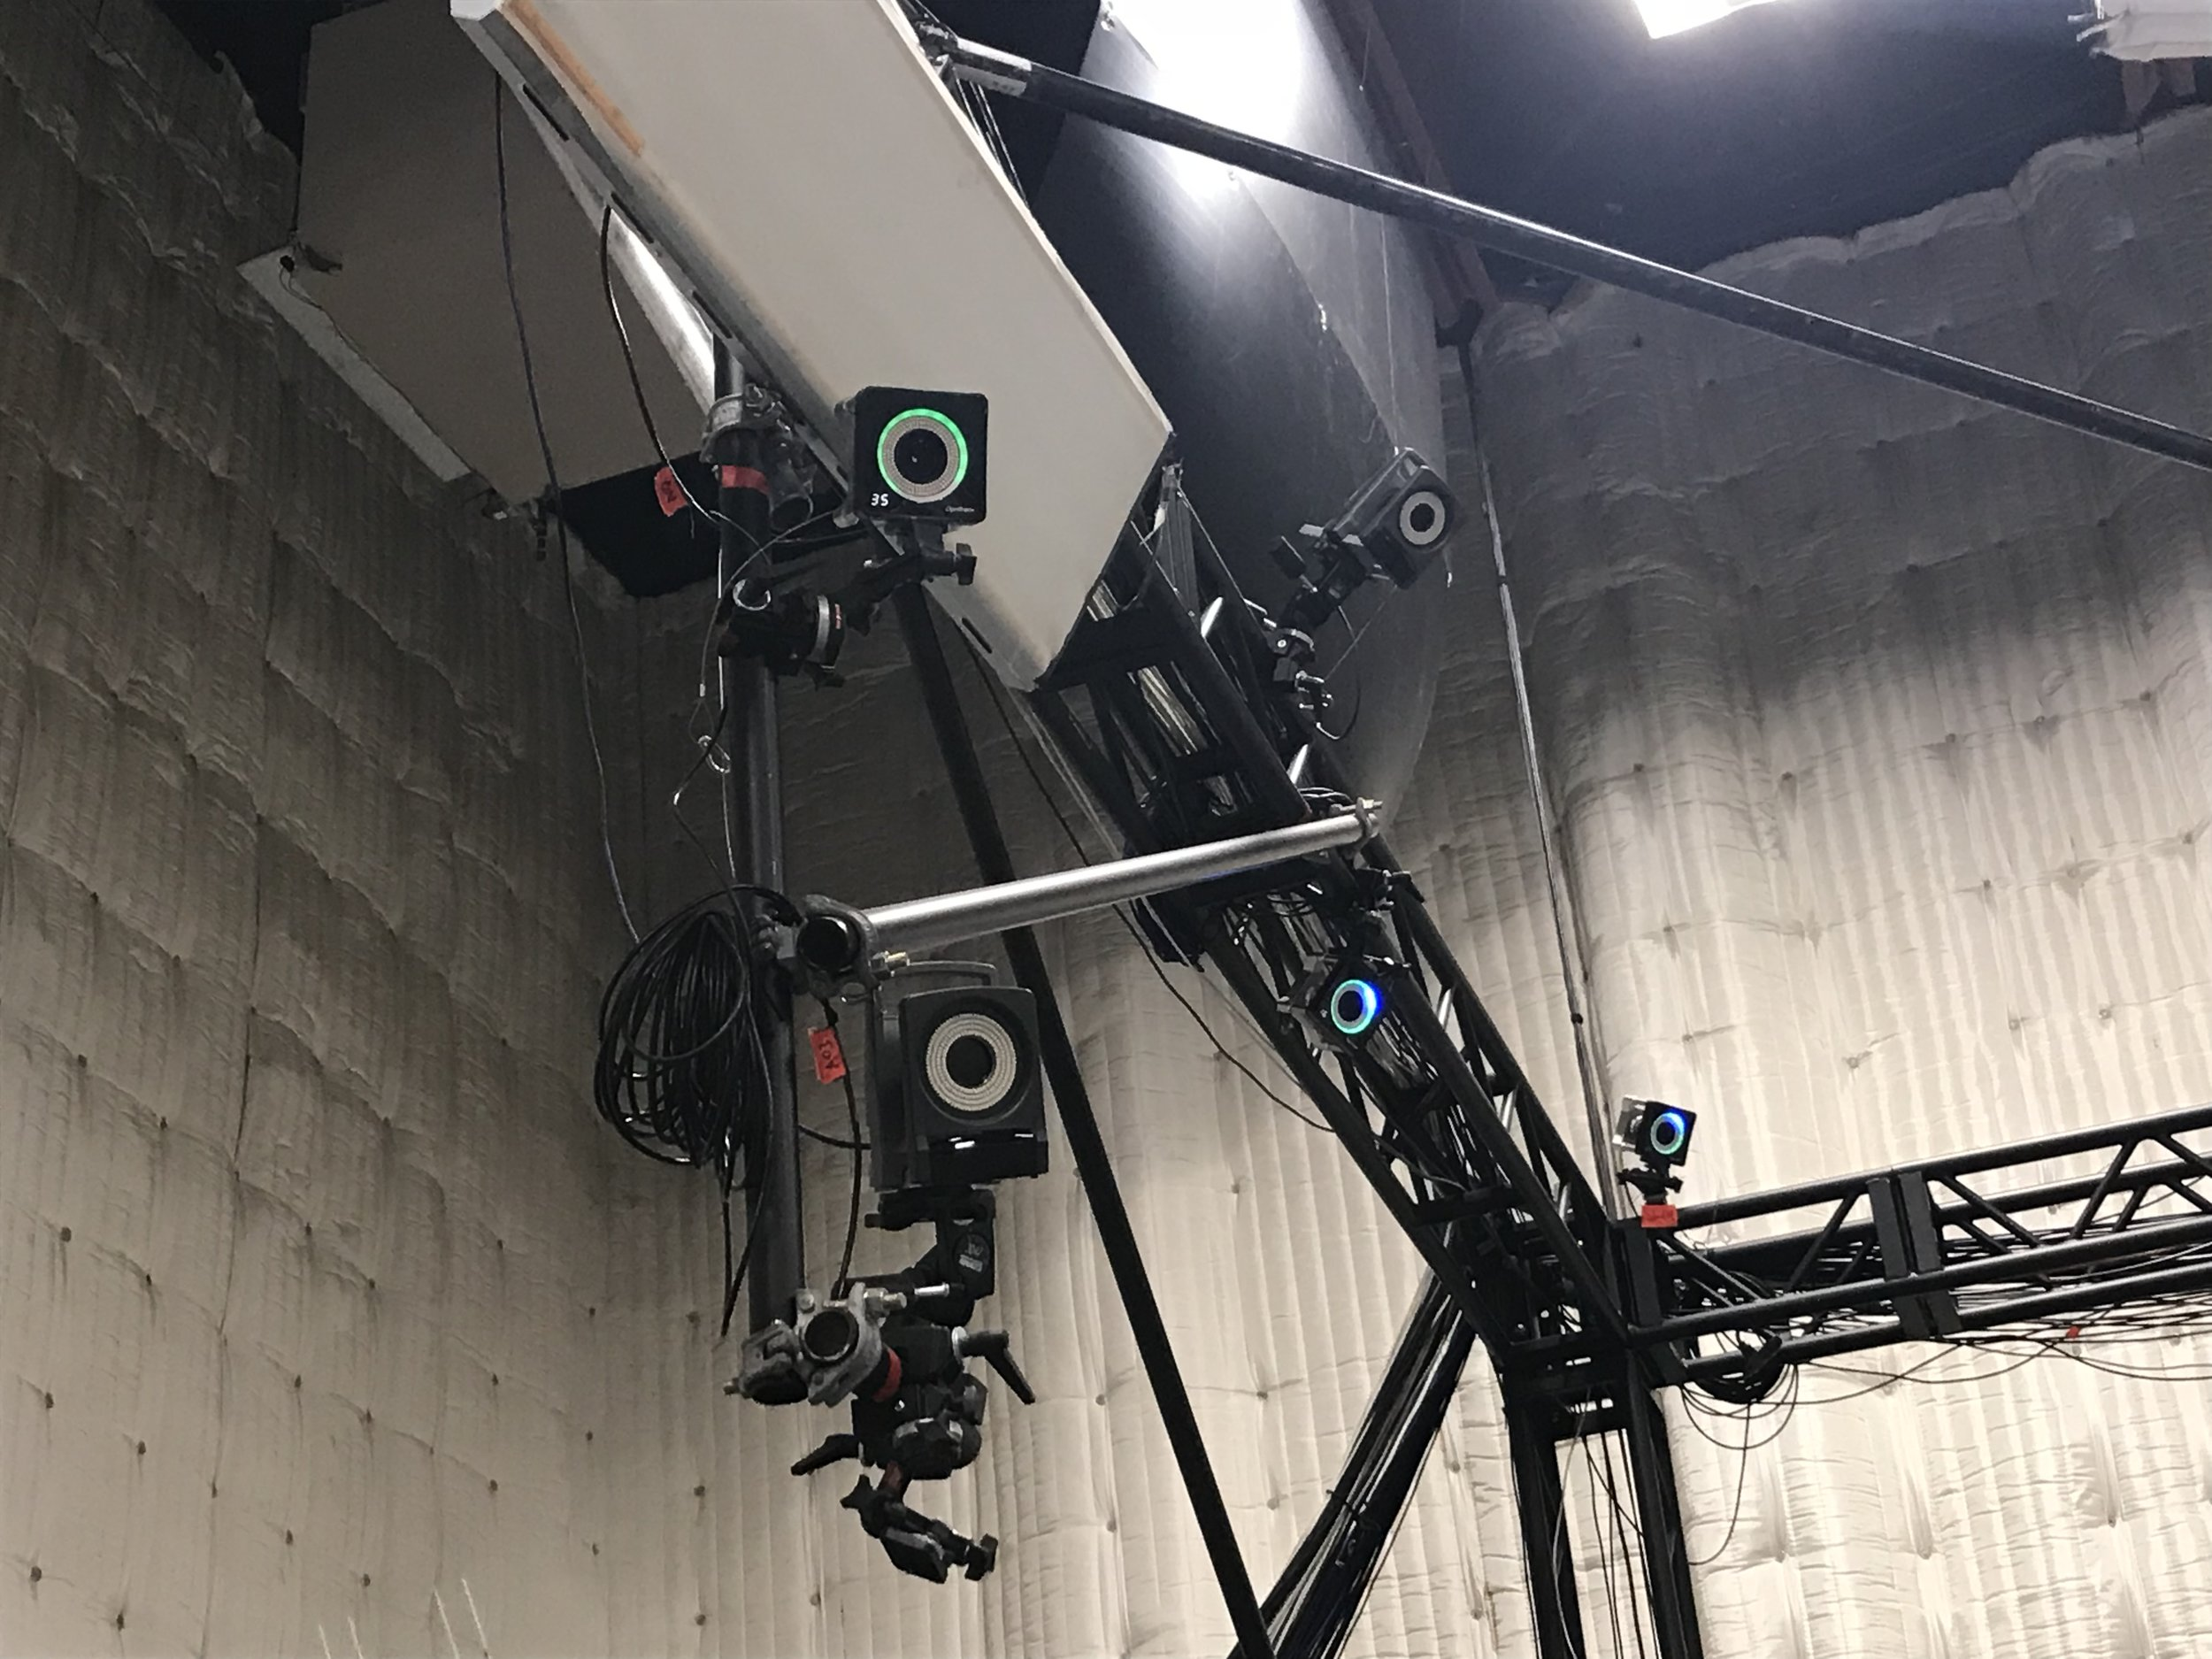
\includegraphics[width=\textwidth]{figures/optitrack.jpg} 
        \caption{Optical tracking system} 
        \label{fig:intro-optitrack} 
    \end{subfigure} 
    \hfill
    \begin{subfigure} [b]{0.46\textwidth} 
        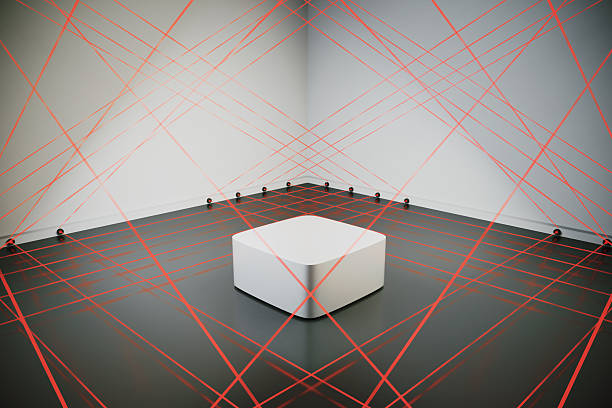
\includegraphics[width=\textwidth]{figures/laser.jpg} 
        \caption{Laser system} 
        \label{fig:intro-laser} 
    \end{subfigure} 
\end{figure}

The deployment of sensors is not limited only to deploying sensors static to the ground.
A notable example is the advent of self-driving cars.
On top of those autonomous vehicles, sensor systems are indispensible for obstacle avoidance and interactions between vehicles.
Tesla (~\ref{fig:intro-tesla}) uses 12 ultrasonic sensors 
near the front and rear bumper 
and later changed into a vision system with only cameras 
\footnote{\url{https://www.tesla.com/en_eu/support/transitioning-tesla-vision}}. 
And TuSimple, an autonomous truck company, employs a combination of cameras, radars and lidars 
for their perception system \footnote{\\\url{https://www.tusimple.com/blogs/tusimple-1000-meter-perception-system}}. 

\begin{figure}[ht] 
    \centering 

    \begin{subfigure}[b]{0.49\textwidth} 
        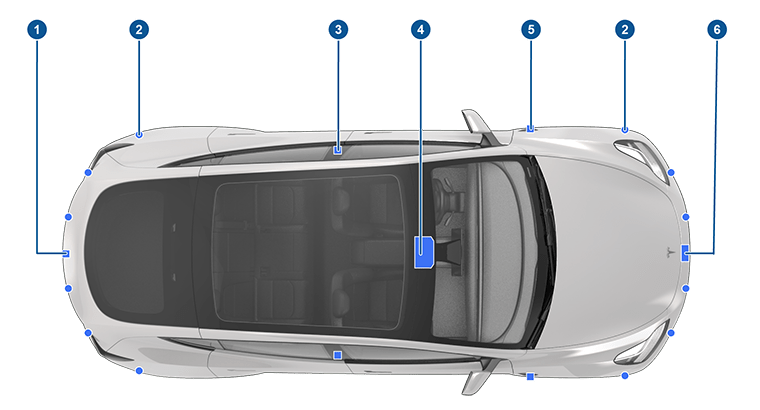
\includegraphics[width=\textwidth]{figures/tesla.png} 
        \caption{
        Tesla model Y's sensing system
        equipped with cameras (\circled{\small{1}}, 
        \circled{\small{3}}, 
        \circled{\small{4}}, \circled{\small{5}}),
        ultrasonic sensors \circled{\small{2}}, and a radar \circled{6}.
        }
        \label{fig:intro-tesla} 
    \end{subfigure} \hfill
    \begin{subfigure}[b]{0.4\textwidth} 
        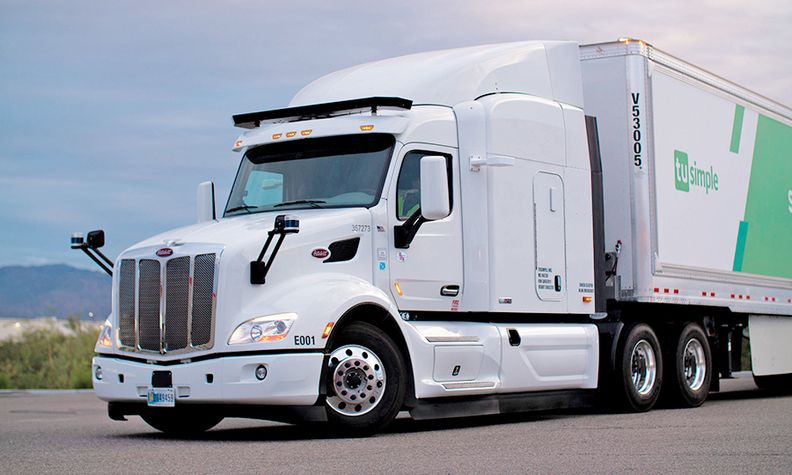
\includegraphics[width=\textwidth]{figures/tusimple.jpg} 
        \caption{TuSimple autonomous truck equipped with CMOS long-range cameras, 
        LiDARs and radars} 
        \label{fig:intro-truckcam} 
    \end{subfigure} 
    \caption{Sensor systems on autonomous vehicles}
    \label{fig:intro-autonomous-vehicles}
\end{figure} 

The placement of sensors are extremely crucial for many reasons.
First, a typical high-frequency tracking camera can cost up to serveral thousands US dollars in 2023, 
let alone sensors with specific industrial or millitary purposes. If a certain sensor layout solution
can reduce the number of sensors used in, e.g., in a security environment, autonomous vehicle, or in a patrolling robot,
the cost for deployment of such sensor systems can be greatly reduced.
Second, real sensors come with many characteristics as mentioned in \cite{sebastian2005prob},
range sensors can have noise, unexpected objects blocking the view, sensing failures, random measurements and so on.
Hence, the objective that a sensor system being more balanced in terms of work load is a reasonable assumption
when quality assurance and fault tolerance are the main concerns for the system. 
Lastly, a good sensor deployment in systems like surveilence camera system means less human labor from the security personel,
and less ernergy consumpsion.
\section{Background}
In this section, we provide sufficient background knowledge and terms used in this dissertation, 
they will be used without explaination in the following chapters. 

\subsection{NP and NP-hardness}
% In the area of optimization, which this thesis is focusing on, NP-hardness has the 
% The definitions are taken from \cite{vazirani2001approximation}
\begin{definition}[NP]
    A language $L\in NP$ if there is a polynomial $p$ and a polynomial time bounded Turing machine M, 
    called the {\textit verifier}, such that for each string $x\in \{0, 1\}^*$: 
    \begin{itemize}
        \item if $x\in L$, then there is a string $y$ (the certificate) of polynomially bounded length, i.e., $|y| \leq p(|x|)$,
        such that $M(x, y)$ accepts, and 
        \item if $x\notin L$, then for any string $y$, such that $|y|\leq p(|x|)$, $M(x,y)$ rejects.
    \end{itemize}
\end{definition}

A colloquial way in \cite{vazirani2001approximation} to describe an NP is the class of problems that have ``short and quickly verifiable'' 
Yes certificates.
% NP-complete problems refers to the class of problems such that every problem in NP can be reduced to it.
And NP-hard problem is the class of problems such that every problem in NP can reduce to it.
Typically, when we call an optimization problem NP-hard, it means the decision version of it is NP-hard.
\subsection{Integer programming}
Since most natural optimization problems are NP-hard, mathematical programming tools are often 
used for solving the problem for its generality and efficiency. Essentially, they take in
some mathematical models including a set of variables $x_1, \dots, x_n$ and a set of constraints,
\begin{align*}
    a_{11} x_{11} + \dots + & a_{1n} x_{1n} \geq b_1,\\
    \dots & \\
    a_{m1} x_{m1} + \dots + & a_{mn} x_{mn} \geq b_m,
\end{align*}
and objective 
\[
    \min a_{11} x_{11} + \dots + a_{1n} x_{1n} \geq b_1.
\]
% e.g., its usage in Multi-robot Path Planning Problem (MRPP) \cite{HanYu19IROS, GuoHanYu21ICRA}, sensor coverage. 
Commercial integer programming tools include Gurobi \cite{optimization2019gurobi} and IBM CPLEX \cite{cplex2009v12}, while open-source 
libraries include SCIP \cite{achterberg2009scip}, CBC \cite{forrest2005cbc}, GLPK \cite{makhorin2008glpk}, and so on. 
Modern tools, even in the open sourced branch, are pretty mature and developed, and hard to optimize within the framework itself. 
\section{Problems Studied in the Dissertation}
In this section, we provide an overview of the problems studied in the later chapters, 
where each chapter can be considered as an independent entity. 

\subsection{Approximation algorithm}
For an optimization algorithm $\Pi$, OPT($\Pi$), or sometimes OPT, 
denotes the optimal solution of the problem instance. An $(1+\alpha)$-OPT or a $(1+\alpha)$-optimal solution refer
to a solution with abjective value of $(1+\alpha)$OPT for a minimization problem. 

\begin{figure}[h]
    \centering
    \begin{subfigure}[b]{0.4\textwidth}
        \centering
        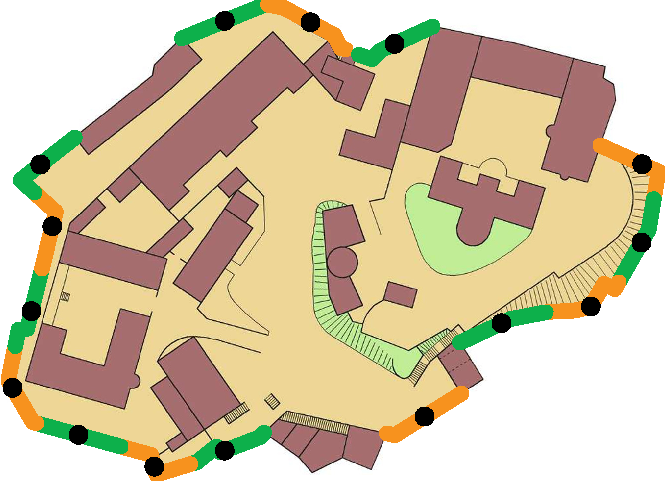
\includegraphics[width = \textwidth]{chapters/opg/figures/castle_15-eps-converted-to.pdf}
        \caption{Optimal perimeter guarding with homogeneous sensors}
        \label{fig:intro-opg-ho}
    \end{subfigure}
    \begin{subfigure}[b]{0.4\textwidth}
        \centering
        \reflectbox{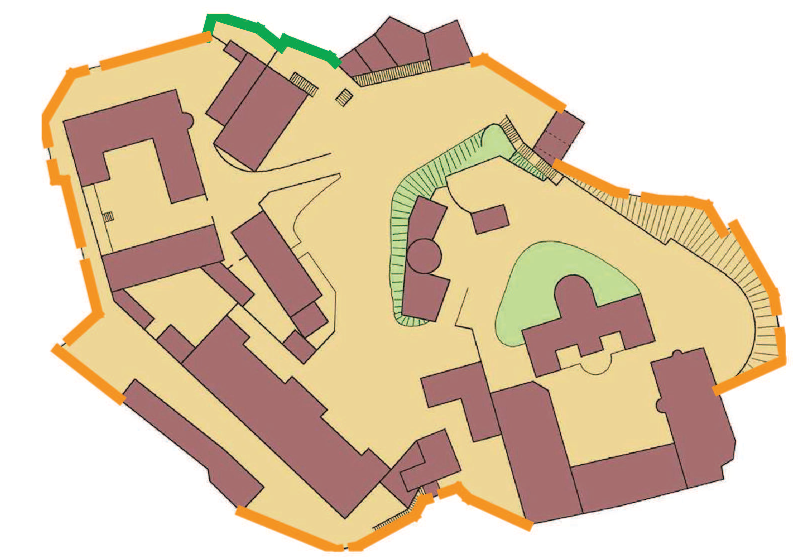
\includegraphics[width = \textwidth, angle=180]{chapters/opg-ext/figures/opgmc-castle-thin-eps-converted-to.pdf}}
        \caption{Optimal perimeter guarding with heterogeneous sensors}
        \label{fig:intro-opg-he}
    \end{subfigure}
    \caption{Optimal perimeter guarding}
    \label{fig:intro-opg}
\end{figure}


The first set of problems we studied relate to optimally assigning a larger number of sensing
robots (or other types of autonomous agents) to guard the perimeters of closed 2D regions,
where the perimeter of each region to be guarded may contain multiple disjoint polygonal chains.
Each robot is responsible for guarding a subset of the perimeter and any perimeter must be guarded
by at some robot.
The sensing range of each robot is assumed to be a continous line on top of the perimeter of some regions. 
Specifically, two problems will be introduced, perimeter guarding with homogeneous sensors (~\ref{fig:intro-opg-ho}),
and with heterogeneous sensors (~\ref{fig:intro-opg-he}). 
The homogeneous case can be solved using only classical algorithms. 
While the heterogeneous case is NP-hard, but can still be solved with dynamic programming under a reasonable
amount of time. 


\begin{figure}[h]
    \centering
    \begin{subfigure}[b]{0.4\textwidth}
        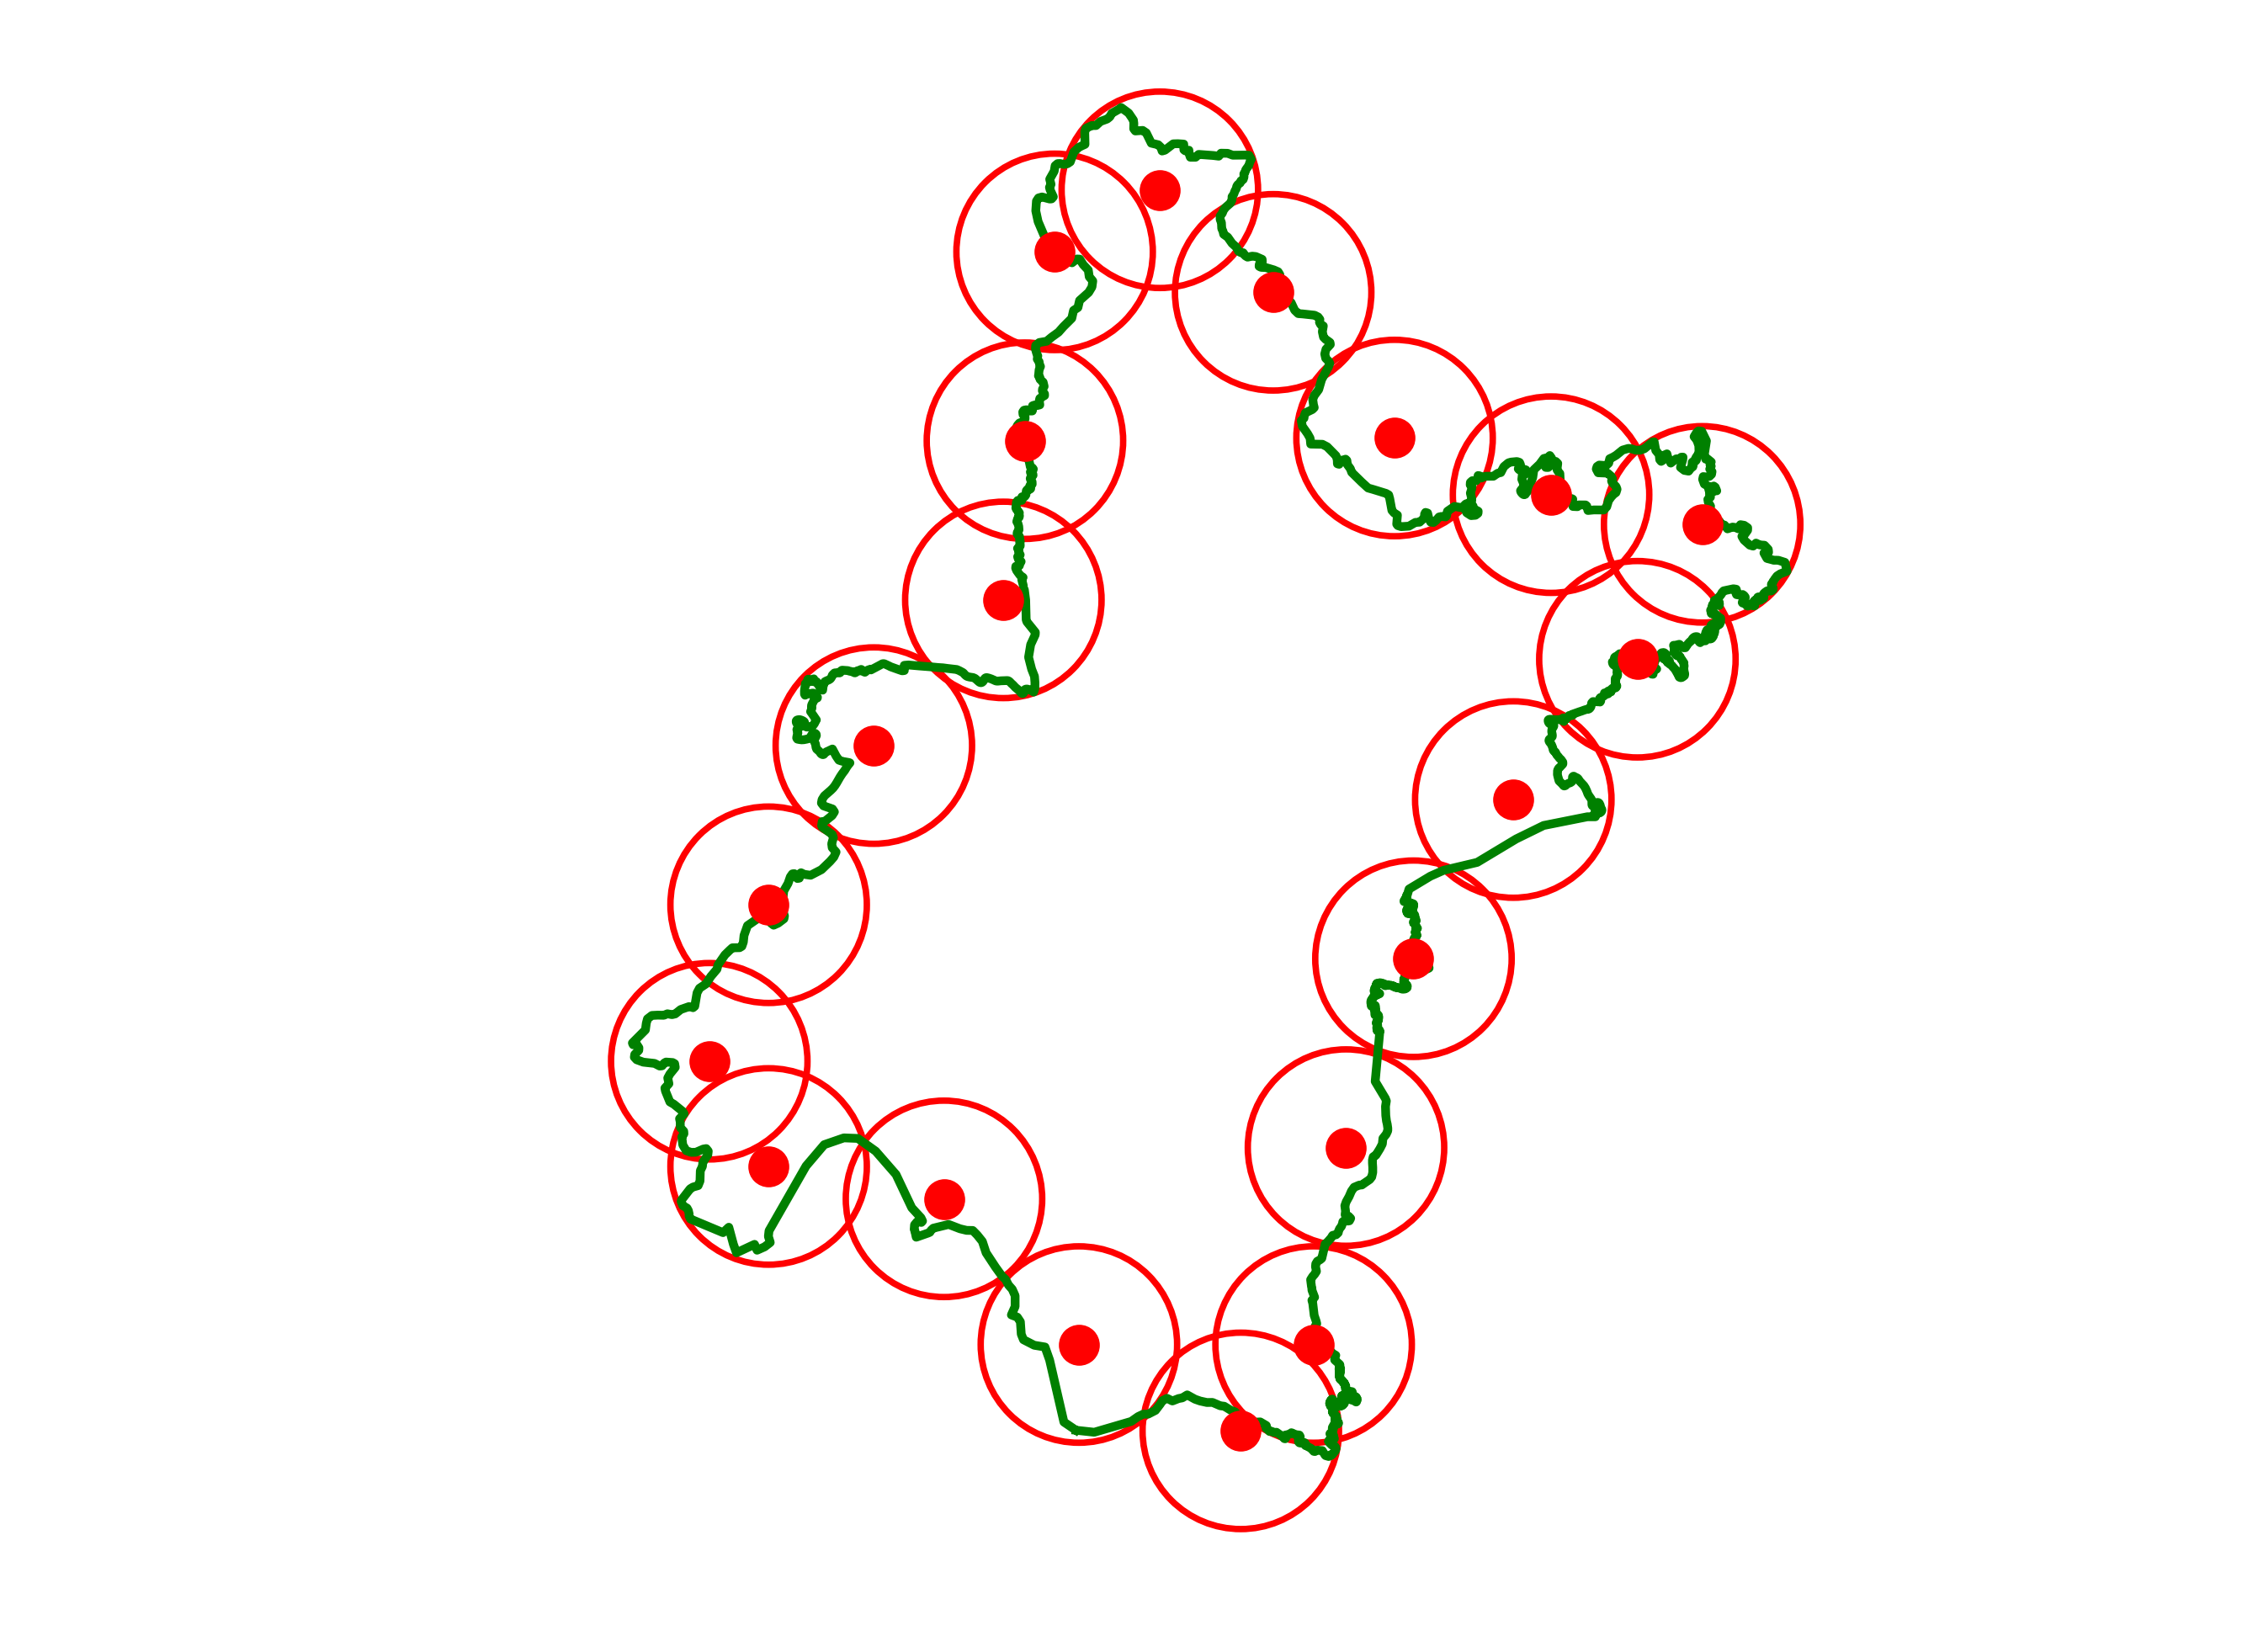
\includegraphics[width = 1.2\textwidth]{chapters/osg/figures/wuhan_ilp.png}
        \caption{Optimal perimeter guarding with 2D range sensors}
        \label{fig:intro-opg2d}
    \end{subfigure}
    \begin{subfigure}[b]{0.4\textwidth}
        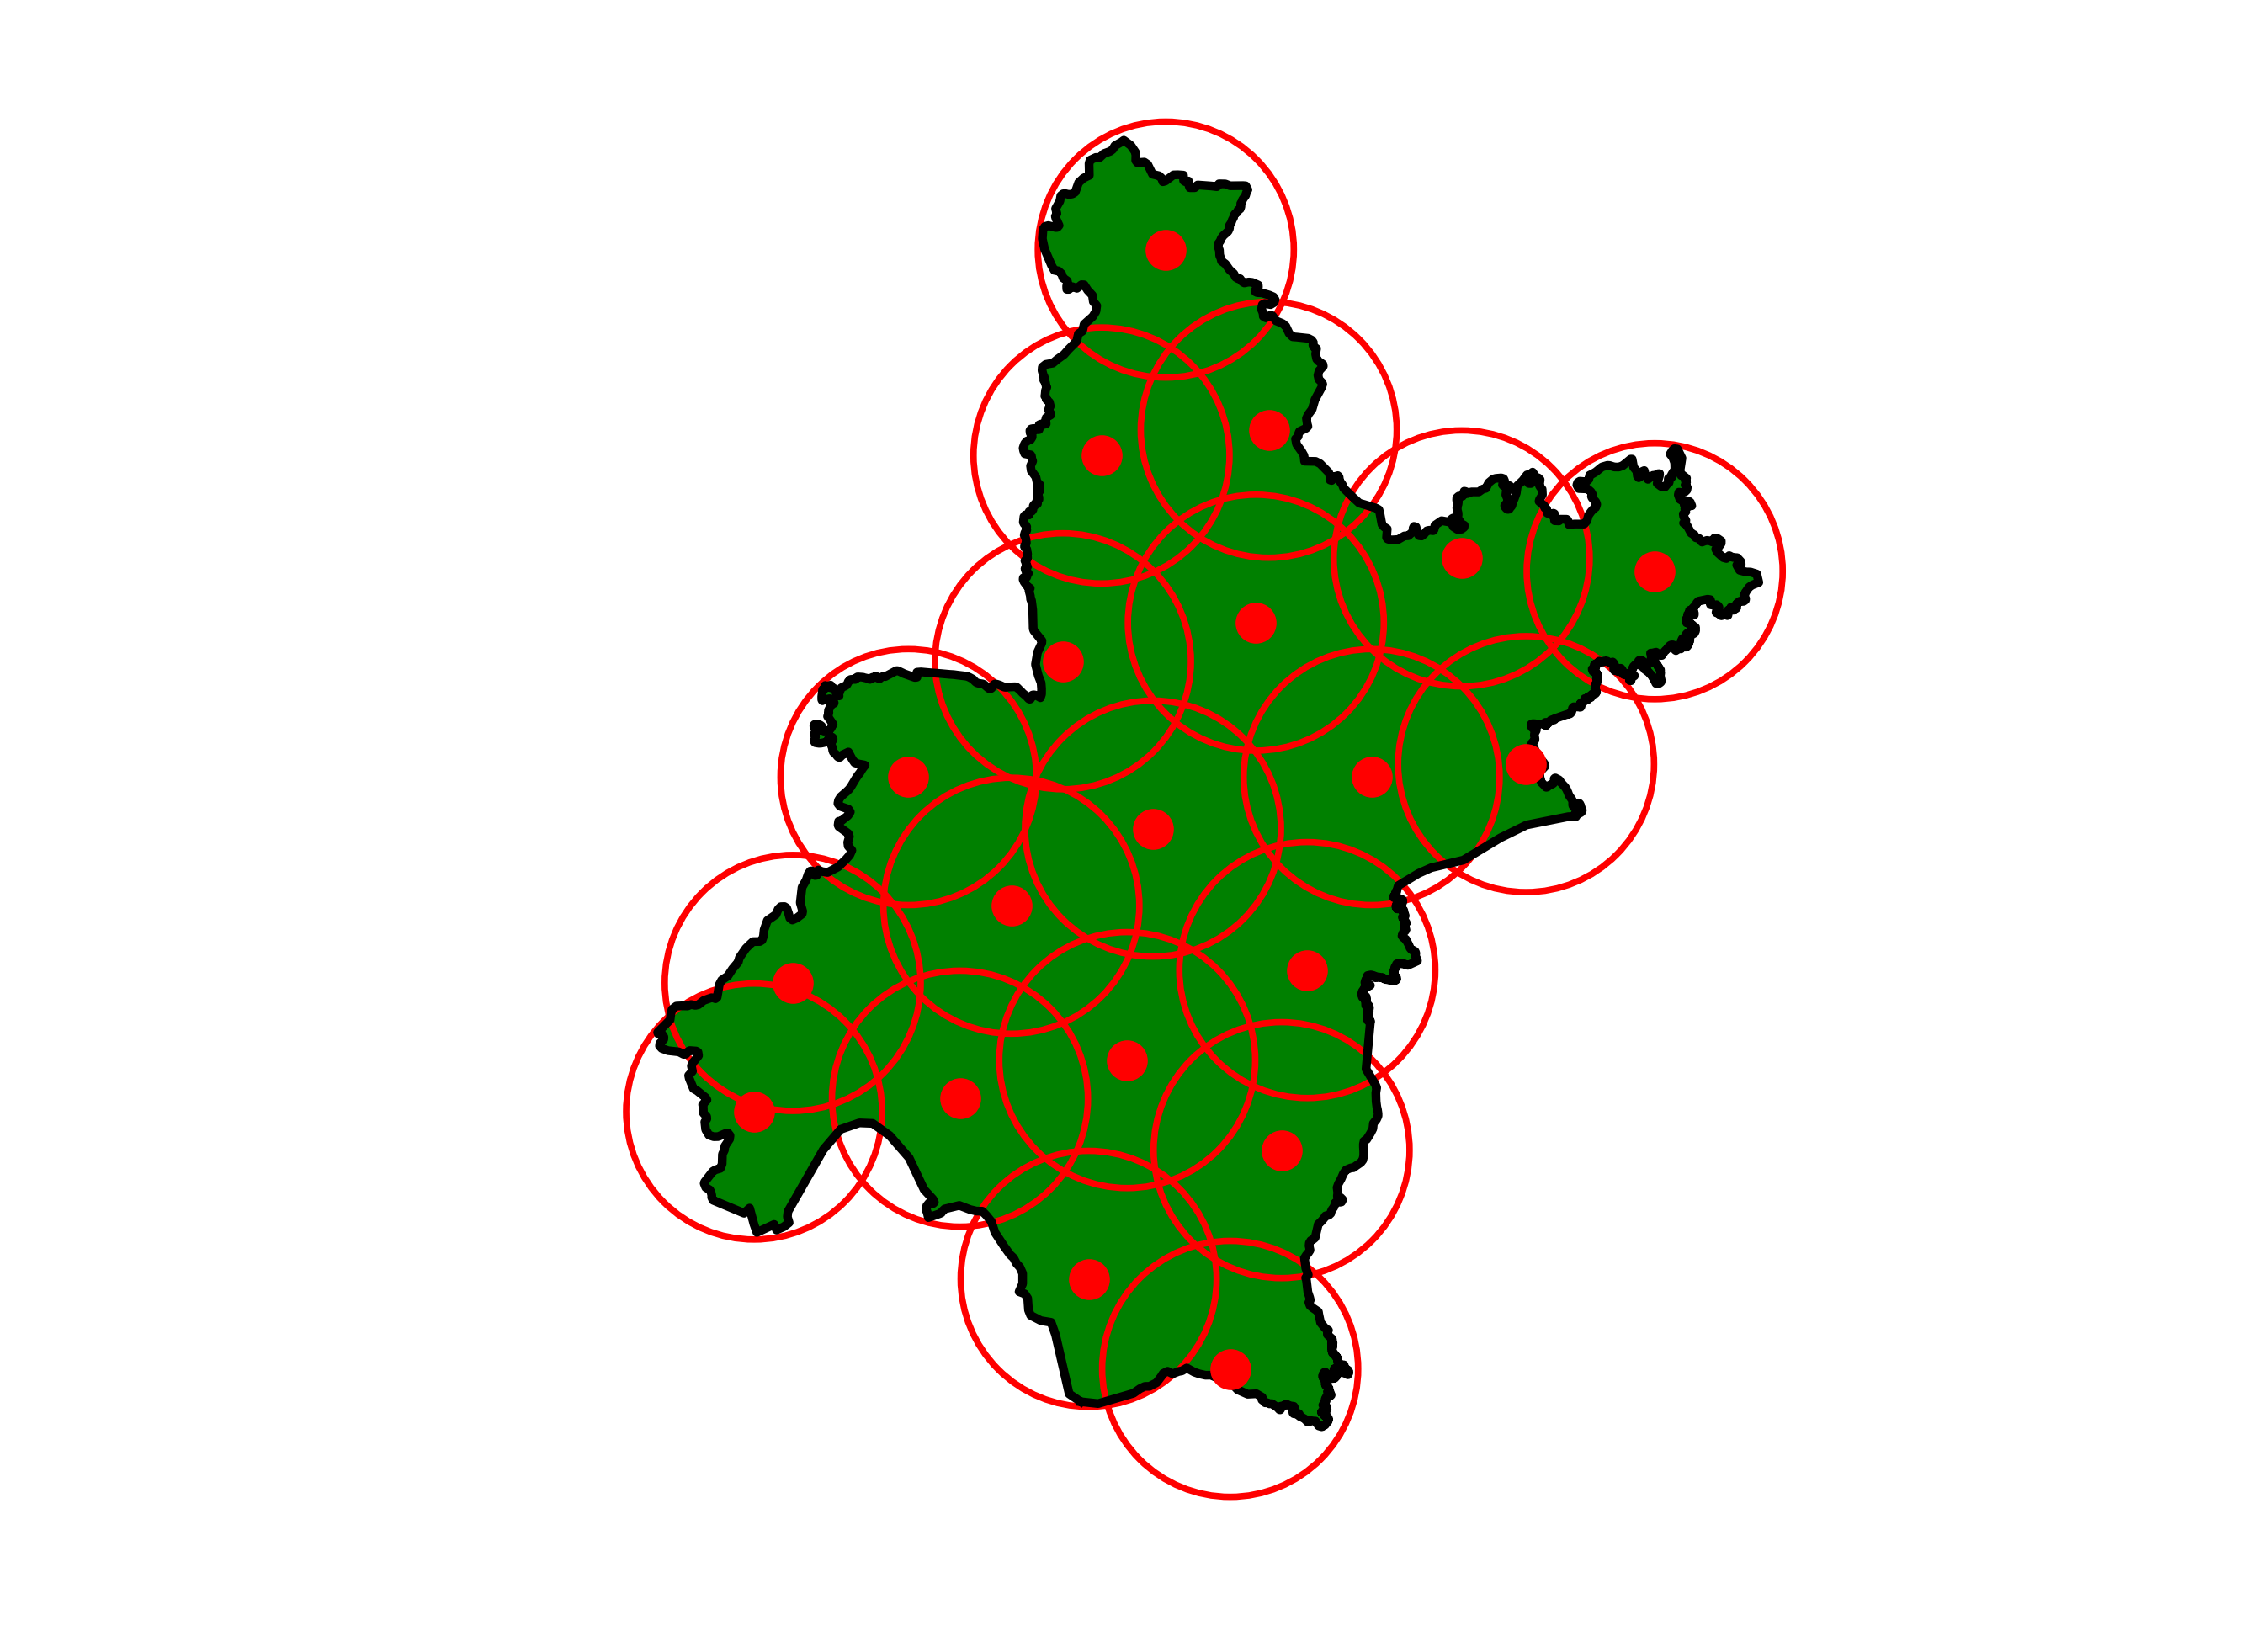
\includegraphics[width = 1.2\textwidth]{chapters/osg/figures/wuhan_region_ilp.png}
        \caption{Optimal region guarding with 2D range sensors}
        \label{fig:intro-org2d}
    \end{subfigure}
    \qquad
    \qquad
    \caption{Optimal set guarding with 20 sensors to cover the perimeter and interior of some region}
    \label{fig:intro-osg}
\end{figure}
Then, we continues with perimeter guarding but uses 2D circles to represent the 
coverage range of sensors. The study extends to guarding 2D regions beyond the perimeters. 
When given a bounded $\mathbb R^2$ to be guarded, and $k$ mobile sensors with variable sensing range of $r_i$, 
our objective is to minimize $\max r_i$.
Our study shows that even for covering the boundary or interior of a simple polygon, 
the problem of find the minimum sensing radius is NP-hard to approximate within a factor of 1.152, e.e.,
unless P=NP, there is no polygnomial solution for finding a $1.152$ optimal solution. 
However, on the side of computational method, a fully polynomial time approximation algorithm 


\begin{figure}[h]
    \centering
    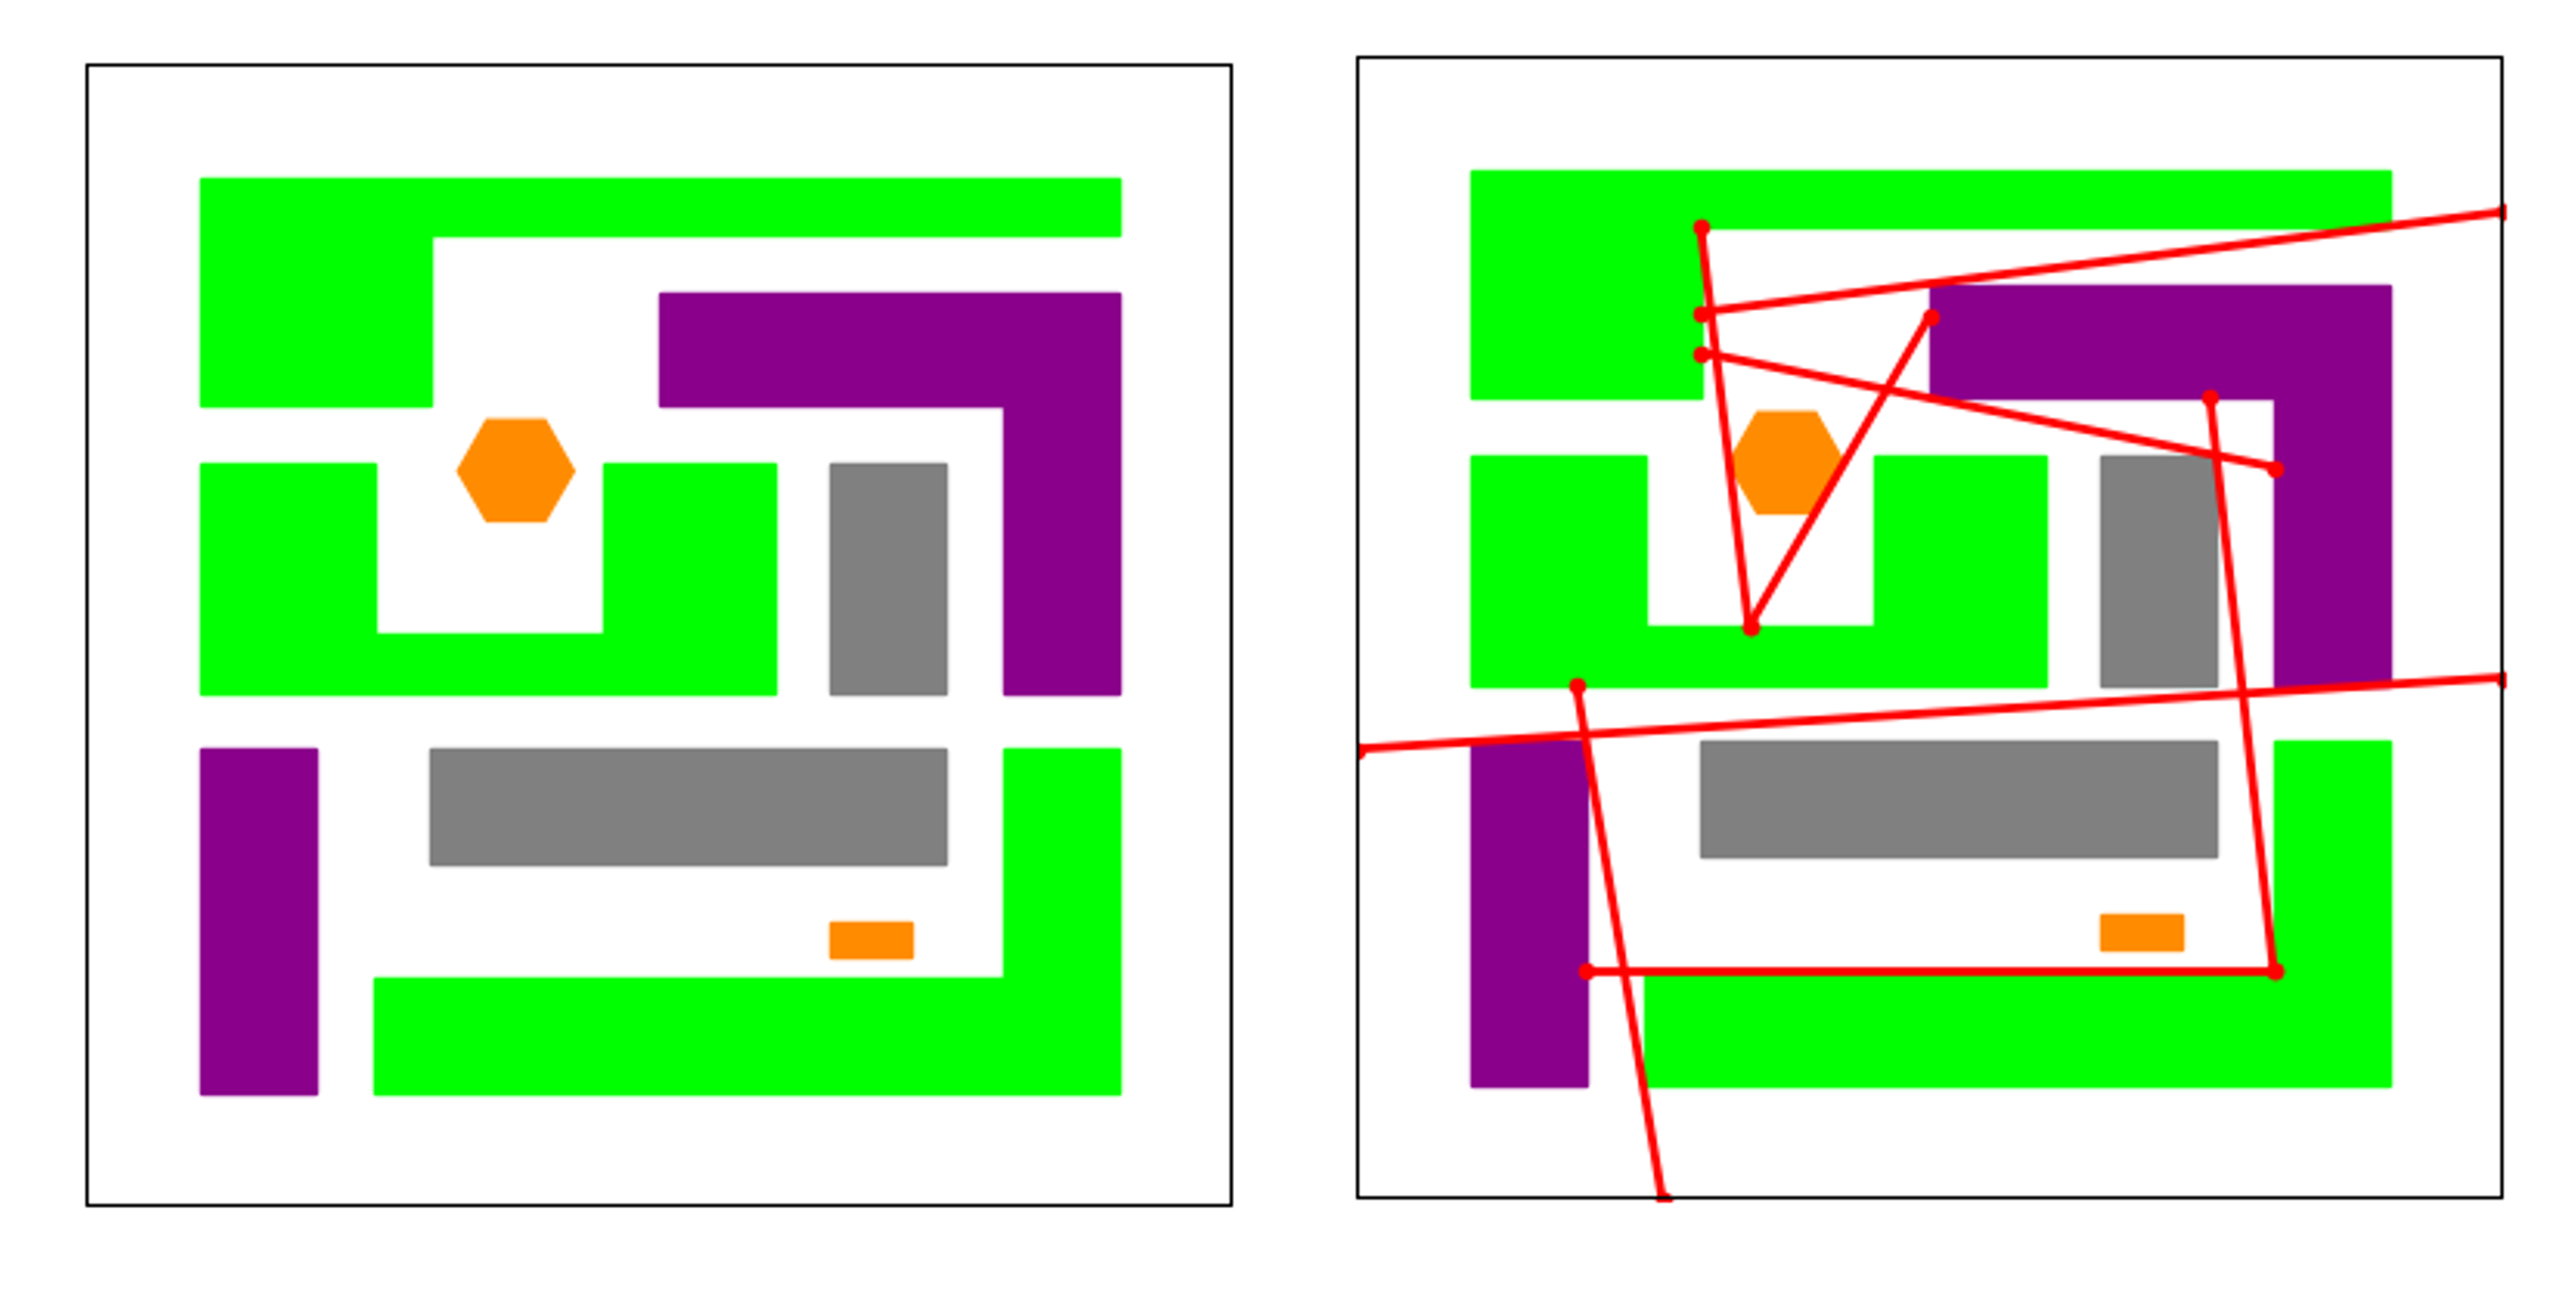
\includegraphics[width = 0.5\textwidth]{chapters/bf/fig/intro_pic.png}
    \caption{Separating three sets of building blocks (orange, purple and green) with the existence of two grey obstacles.}
    \label{fig:intro-lines}
\end{figure}


After two chapters's discussion on covering perimeters or regions, which is essentially separating 
some crtical polygonal regions from the outside workspace. 
The fourth chapter digs deeper into this problem by studying the separation of more than two regions. 
To simplify the problem, a line-of-sight sensing model will be adopted, where each sensor can cover
an unobstructed line segment like a laser beam. Also, the regions are assumed to be polygonal.
The objective in this case is to minimize the number of sensors used to separate these polygonal sets 
at the existence of obstacles (see ~\ref{fig:intro-lines}).
% The main objective here is to minimize the number of sensor used.
The problem is NP-hard even for the problem of separating two sets of regions with the minimum number of lines. 
Still, integer programming can provide a near-optimal solution for around 20 objects in a reasonable amount of time. 

\begin{figure}[h]
    \centering
    \vspace{-.8in}
    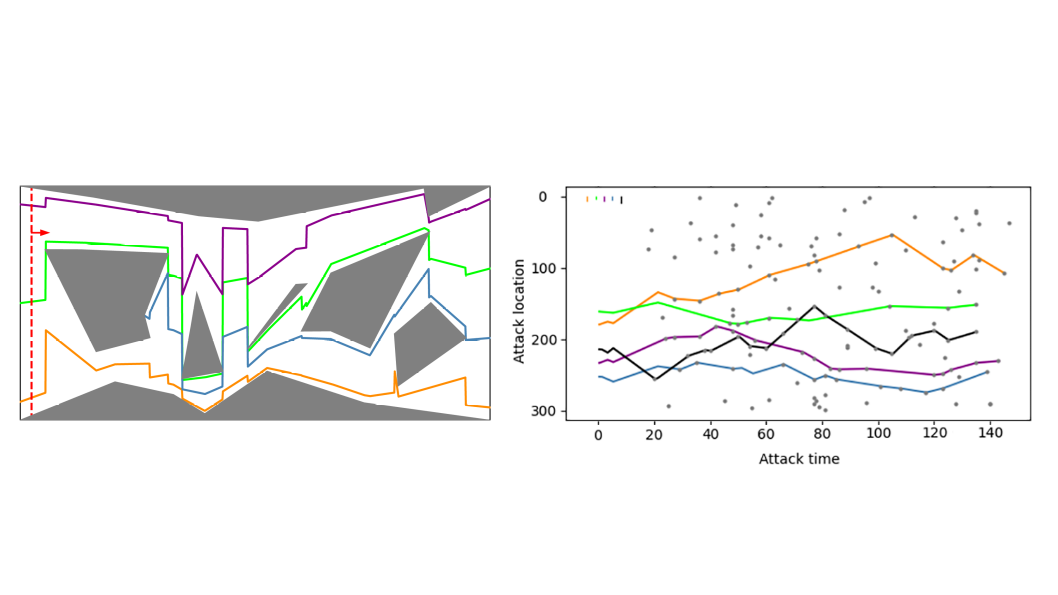
\includegraphics[width=.8\textwidth]{figures/dynamic-intro.png}
    \vspace{-.5in}
    % {
    %     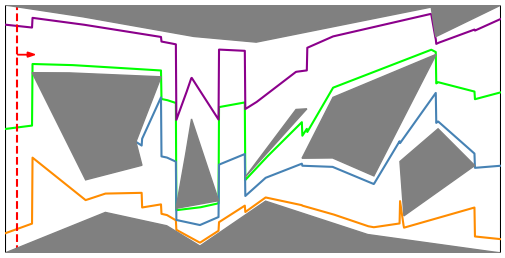
\includegraphics[width = 0.35\textwidth]{chapters/sc/fig/instance_2.png}
    % }
    % 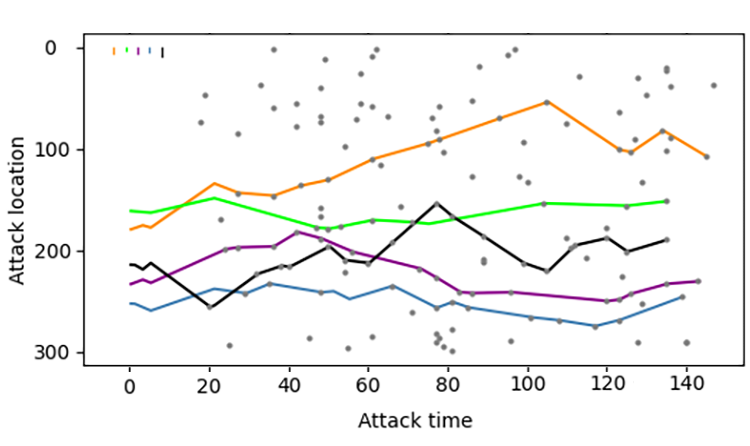
\includegraphics[width = 0.35\textwidth]{chapters/bd/fig/inf_horizon_example-v.png}
    \caption{[left] the coordinated sweeping problem, [right] the perimeter defense problem.}
    \label{fig:intro-bd-sc}
\end{figure}

The fifth chapter duels with the dynamical setting for mobile sensing robots, 
and two different but related problems are studied. 
The first problem is the boundary defense problem in the context of heterogeneous defenders first studied in \cite{adler2022role}.
It can be seen as an extension of the perimeter defense probelm \cite{shishika2020review}. 
In this problem, there are $k$ sensing robots moving on top of a perimeter with different speeds $v_1,\dots,v_k$.
A sequence of attacks $\langle loc_i, t_i \rangle_{i=1}^{n}$ are given at different time stamps and at different locations.
The objective is to intercept as many attacks as possible.
The second problem is the coordinated sweeping problem where a group of robots coordinate to sweep a region 
with obstacles. Each robots possess a given sensing capabilities, and the sweeping trajectory is 
given beforehand. The objective of it is to minimize the number of robots used such that the sweep plan 
can be executed and every point in the workspace is sensed with a certain required quality. 

\begin{figure}[ht]
    \centering
    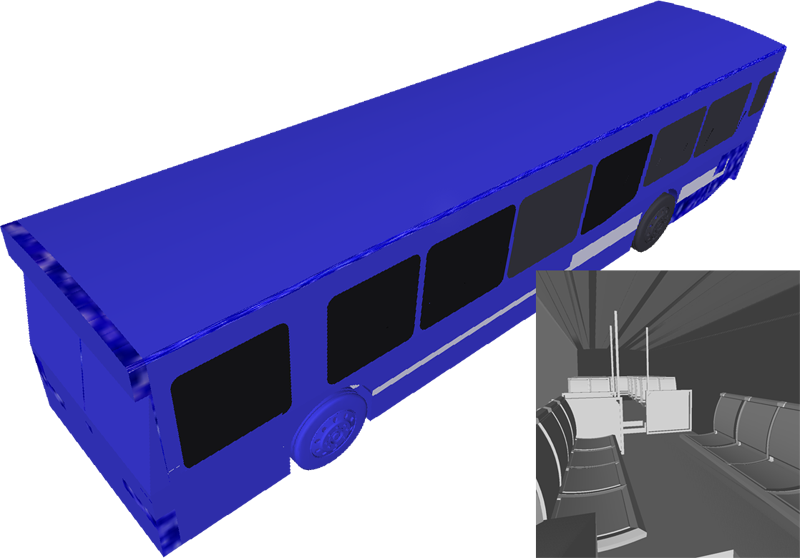
\includegraphics[width = 0.45\textwidth]{chapters/surf/fig/bus.png}
    \hfill
    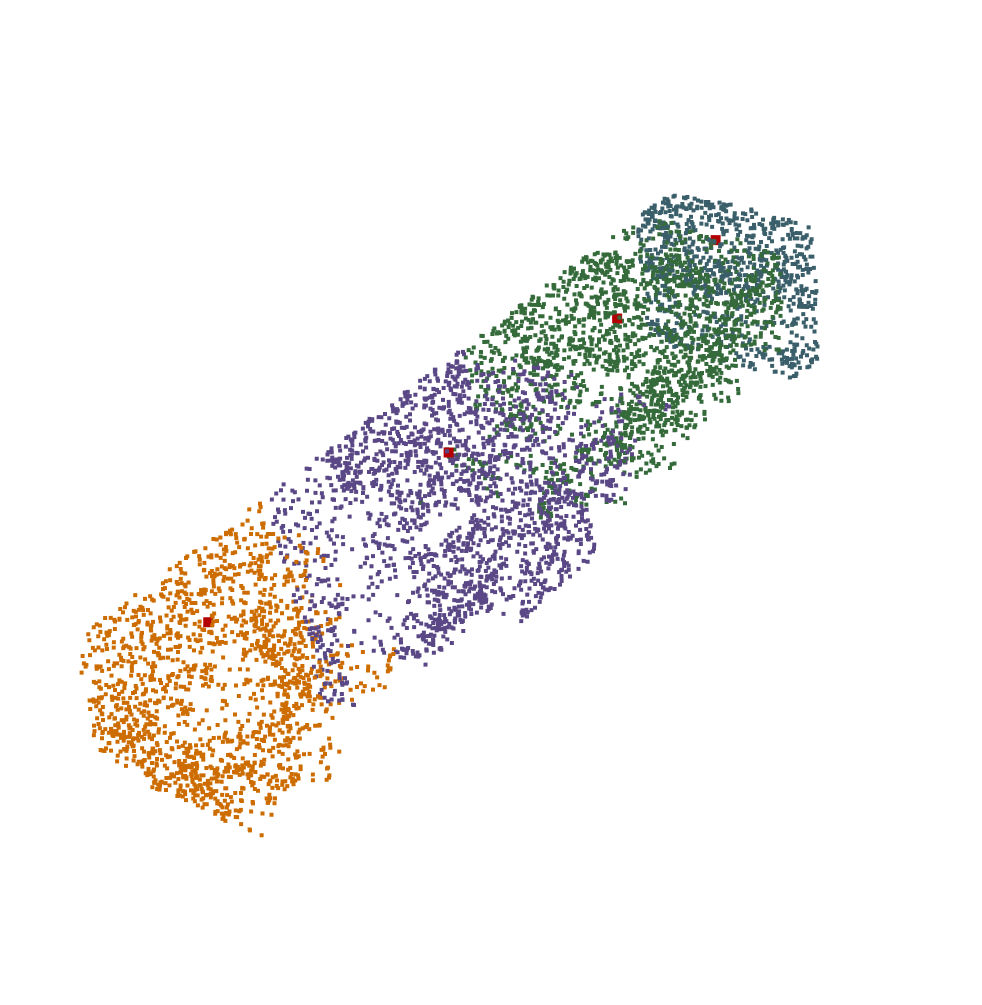
\includegraphics[width = 0.4\textwidth]{chapters/surf/fig/bus_result_3.png}
    \label{fig:intro-surf}
\end{figure}
The sixth chapter dicusses a real-world application on the placement of UV (ultra violet) lights 
to cover the surface of some regions for the sanitization purpose. 

\begin{comment}
\section{Literature review} 
\subsection{Coverage-related problems in computational geometry} 
\subsection{Mobile sensing robot coverage control} 
\subsection{Multi-robot coordination} 
\subsection{Sensor network} 
\end{comment}
